%%%%%%%%%%%%%%%%%%%%%%%%%%%%%%%%%%%%%%%%%%%%%%%%%%%%%%%%%%%%%%%%%%%%%%%%%%%%%%%%
%% CAPITULO
%%%%%%%%%%%%%%%%%%%%%%%%%%%%%%%%%%%%%%%%%%%%%%%%%%%%%%%%%%%%%%%%%%%%%%%%%%%%%%%%
\chapterimage{chapter_head_2.pdf} % Chapter heading image

\chapter{Historia do samba e do batuque}
\index{Historia do samba}
O samba como principal manifestação da cultura brasileira está bem reconhecida no Brasil do seculo XXI;
porem, o caminho da palavra samba, ou da ideia do samba, inicia muito tempo atrás;
pois como mostraremos mais adiante, existiu uma transição entre os termos ``batuque'' e ``samba''.


%%%%%%%%%%%%%%%%%%%%%%%%%%%%%%%%%%%%%%%%%%%%%%%%%%%%%%%%%%%%%%%%%%%%%%%%%%%%%%%%
%%%%%%%%%%%%%%%%%%%%%%%%%%%%%%%%%%%%%%%%%%%%%%%%%%%%%%%%%%%%%%%%%%%%%%%%%%%%%%%%
\section{Cronologia do batuque e o samba}

\begin{tcbremarcar} 
\textbf{Batuque (1800s):}
\index{Batuque!1800s}
\index{Dança!Batuque (1800s)}
\label{ref:batuquedanca1800}

Nos inícios do seculo XIX
se designava com a palavra ``batuque''  a qualquer reunião de ``pretos'' (em expressões próprias da época) realizando danças entendidas como africanas\footnote{
Porem no Brasil existem registros desta palavra desde o século XVIII \cite[pp. 85]{sandroni2001feitico}. }
\cite[pp. 54]{de4danccas} \cite[pp. 73]{lara2007memoria}.
\end{tcbremarcar}
Um exemplo do uso do termo batuque, pode ser visto numa carta ao redator do ``Correio Braziliense''  (Londres, ING),
sobre os negócios públicos em Pernambuco,
escrita no dia 3 de dezembro do 1816, e publicada em 1817 \cite[pp. 468]{batuqueBraziliense},
onde se menciona\footnote{\label{footort}A forma da escrita corresponde ao texto original}:
\begin{citando}%%
Quasi dous annos depois, o Ouvidor das Alagoas, que não tinha tido parte neste Drama,
sonhou com outro levante de pretos na sua comarca, 
fundamentado unicamente em um \textbf{batuque} de dança, 
que alguns faziam nas immediaçoens de um Engenho de assucar, ...
\end{citando} 
Pelo que se observa, 
a palavra ``batuque'' não se usava para referenciar a uma dança em particular e sim aos festejos dos negros em geral \cite[pp. 85]{sandroni2001feitico}.

\PRLsep{Samba 1830 - 1850}

\begin{tcbremarcar}
\textbf{Origem do termo samba:}
Entre as explicações da origem da palavra ``samba'', 
a mais conhecida, é a que promove que esta vem do idioma quimbundo, 
sendo derivado da palavra ``semba''  que significa umbigada \cite[pp. 32]{jornalsambaderoda2} \cite[pp. 47]{diniz2008almanaque} \cite[pp. 50]{da2015historia}.
Uma referencia muito conhecida deste vinculo é a descrita no livro ``O negro e o garimpo em Minas Gerais''
de Mata Machado Filho, onde ele comenta que ``os negros corrigem para semba se 
alguém lhes fala em samba'' \cite[pp. 85]{sandroni2001feitico}. Assim se vê que existe
desde antanho uma relação entre as palavras, 
samba, semba e umbigada.
\end{tcbremarcar}

Paralelamente na historia, a palavra samba estava iniciando a ser usada como parte
das expressões nestos festejos populares. 
Isto pode ser visto na ordem do dia do Quartel do Governo das Armas em
Pernambuco, 8 de julho de 1830, publicado no jornal ``Diario de Pernambuco''(PE), 
onde se  relata\footref{footort} \cite[pp. 3]{sambadiariodepernanbuco}:
\begin{citando}%%
Naõ existindo fora da Capital nos diferentes pontos,
onde se achão destacadas as Companhias deste Corpo, 
hum serviço ativo, a que sejão ellas forçadas, 
necessariamente a occiozidade dispora' 
aos mais bem conduzidos a se entreterem nas pescarias de curraes e trapaçoens de coqueiros,
em cujos passatempos sera' recebida com agrado a viola, e o \textbf{samba};
e aos peraltas, cada vez os fara' mais dezenvolvidos na conjugação do verbo surripio.
\end{citando}
Anos posteriores podemos encontrar uma dualidade no uso da palavra samba, 
tanto no sentido de música como de dança; por exemplo, no jornal ``O Capuceiro''(PE),
do dia 3 de fevereiro de 1838, temos uma referencia ao samba como música,
onde ademais se ressalta a beleza da interpretação musical;
o seguinte é um fragmento desse texto\footnote{\label{footort2}A forma da escrita corresponde ao texto original} \cite[pp. 1]{sambaperiodicoocapuceiro}:
\begin{citando}%%
Segue se, que tão perfeita na Cantoria era Catalini, ou a Pasta,
como pai Antonio descantando no seu birimbau; que tanto val huma garatuja da China,
que vinhão nos bules, e bandejas,
como as pinturas de Rafael, de Rubens, ou do Corregio;
que tão agradavel he hum \textbf{samba} d'almocreves, como a Semiramis,
a Gaza-ladra, o Tencredi, \&c. de Rossini, ...
\end{citando}
Também podemos achar outra referencia do samba no sentido musical, no jornal ``Diário do Rio de Janeiro''(RJ),
do dia 19 de abril de 1939, onde se menciona\footref{footort2} \cite[pp. 1]{sambadiariorj1}:
\begin{citando}%%
Em quanto o cortezão, o palaciano, o gamenho, o literato, o magistrado etc., 
espancão melanconias, desvanecem cuidados tomando em ricas bocetas o cheiroso rapé;
o laborioso maluto, a quem furtárão o cavalinho (que é a menina dos seos olhos)
depois de affligir-se, e praguejar em balde arranca do quijeje (bolso na celoura)
o encebado cornimboque, saca lhe com estalo e tapadoura, e chafurdando as ventas em duas,
ou trez pitadas mestras da sua torradinha, esquece-se do cavallo, resigna-se com sua sorte,
e com uma viola nas unhas zangarrêa o \textbf{samba} por uma noite inteira.
\end{citando}

Nas duas referencias anteriores, 
podemos ver como o samba está relacionado a momentos de descanso e esparzimento, 
onde as pessoas ao ter um tempo para poder desfrutar da vida,
optam por cantar ou tocar um samba.

Por outro lado, temos uma referencia ao samba relacionando-o com a dança, no jornal ``O Capuceiro''(PE),
do dia 12 de novembro de 1842\footnote{Só 6 anos apos referenciar o samba como música, 
no mesmo jornal, é usado o mesmo termo agora relacionado com a dança.}, 
onde mencionam\footref{footort2} \cite[pp. 5]{sambaperiodicoocapuceiro2}:
\begin{citando}%%
Aqui pelo nosso mato,\\
Qn'stava então mui tatamba,\\
Não se sabia outra cousa,\\
Senão a \textbf{dansa do samba}.
\end{citando}
Neste ultimo texto vemos que ainda se diz a \textbf{dança do samba} e não dançar o samba,
mas é possível observar como o termo vai se fusionando com a dança.
Seguindo esta linha de pensamento, 
podemos ver outro exemplo no Jornal ``O Guaycuru''(BA), do dia 26 de maio de 1846,
onde podemos ler o seguinte texto\footref{footort2} \cite[pp. 2]{sambaperiodicooguaycuru}:
\begin{citando}%%
Todavia o famigerado Salles, sem respeito algum aos institutos de sua ordem, 
foi-se pòr na Cachoeira a divertir talvez \textbf{dançando o samba}...
Que bello exemplar da vida religiosa!?
\end{citando}
Como tem sido visto, 
para esta data já se podia ver como as pessoas entendiam o samba como uma dança.
Porem, não terá que se esperar muito pra achar referencias mostrando ao samba
como uma expressão cultural em si mesma, 
uma declaração deste tipo pode ser achada no jornal ``O Cosmorama na Bahia'' (BA), 
no dia 15 de dezembro de 1849, onde menciona\footnote{\label{footort3}A forma da escrita corresponde ao texto original} \cite[pp. 2]{sambaperiodicoocosmorama}:
\begin{citando}%%
Cousa já muito antiga para engordar os patinhos. 
Para o espectaculo seguinte haverá um \textbf{SAMBA} á moda da Bahia, 
em que entram os negreiros todos.
\end{citando}

\PRLsep{Samba por batuque  1887 - 1910}


A emigração ao Brasil, acontecida como fenômeno em massa   entre 1887 e 1902,
o consequente aumento demográfico do país \cite[pp. 18]{trento1989outro}, e 
a abolição da escravatura no Brasil o 13 de maio em 1888 \cite[pp. 117]{dorigny2019abolicoes},
contribuiu, de modo fundamental à modificação do ritmo de vida das comunidades
afrodescendentes no Brasil.
Dado que para o escravo liberto, o trabalho era uma marca indigna ou desonrosa;
pelo qual, este não usava  o único instrumento que tinha, sua força de trabalho, 
para  integra-se na sociedade crescente pôs abolicionista; 
sendo a possibilidade do ócio, a recompensa tão antigamente esperada, 
de modo que o escravo liberto tende a produzir apenas o suficiente para subsistir,
usando o mínimo esforço possível \cite[pp. 28]{durham1966assimilacao} \cite[pp. 25]{trento1989outro}.

Esta tendencia tem um reflexo, na visão que tem a sociedade sobre as expressões,
culturais dos escravos libertos; Por exemplo no jornal ``Gazeta de Noticias'' (RJ), 
no dia 15 de fevereiro de 1890,
no código de posturas - Intendência Municipal, 
na seção 4 sobre, 
``Vozeiras nas ruas e praças, injurias, obscenidades, 
actos contra a moral, tocatas, ajuntamentos, batuques, sungús, cartomancia e adivinhação,
curativos por meio de imposturas'', se menciona\footref{footort3} \cite[pp. 4]{batuqueperiodicogazetanoticias}:
\begin{citando}%%
Art. 259. É prohibido, dentro das casas ou chacaras, o brinquedo chamado \textbf{batuque},
com toques de tambor, cantorias e dansas. Penas: multa de 10\$ e o dobro e cada reincidencia.
\end{citando}
Assim, a realização do batuque, era considerado ao mesmo nível que injurias, 
obscenidades e atos contra a moral, 
pelo que pouco a pouco estas expressões iriam sendo separadas da sociedade,
sendo a norma antes mencionada, e a difícil integração em sociedade do escravo liberto, 
promotores desta tendencia. 

Porem, não todas as expressões culturais de ``pretos'' eram proibidas,
podemos ver só dois dias depois uma referencia ao \textbf{samba}, num contexto diferente; 
no mesmo jornal, 
no dia 17 de fevereiro de 1890, com o título ``Fenianos''
se menciona\footref{footort3} \cite[pp. 1]{batuqueperiodicogazetanoticias2}:
\begin{citando}%%
Não ha adectivos, não ha mesmo na 
rhetorica palavras bombasticas que se 
possam empregar para dizer com a
verdade que o caso exige o que foi o baile
de ante-hontem no Club dos Fenianos.

Cruzavam os salões, socios e convidados
na maior parte fantasiados, dando
muitos d'aqueles sortes de fazer rir até
o mais casto e puro Santo Antonio, que se
lá tivesse entrado persuadido de chamar
as ovelhas desgarradas ao apriseo, teria
cahido no \textbf{samba} como os outros moriaes.
\end{citando}%%
Assim, é possível ver que existe um marcada diferencia de percepção da sociedade, entre o samba e o batuque,
como expressões culturais; e como a primeira, 
iniciou por esses anos seu caminho para subsistir à segunda como a palavra que englobasse às
expressões culturais, antes entendidas como de pretos. 




Anos posteriores podemos ver como dentro do consciente coletivo, 
de uma sociedade em constante mistura racial, 
pode-se escutar em palavras de alguns membros desta,
um chamado ou uma lembrança destes festejos antes tão comuns.
Por exemplo, no jornal ``A Cigarra'' (RJ), 
no dia 16 de maio de 1895, se menciona\footnote{\label{footort4}A forma da escrita corresponde ao texto original} \cite[pp. 2]{batuqueperiodicoacigarra}:
\begin{citando}%%
Fosse eu um homem menos dado 
ao cumprimento do dever e estaria a 
esta hora, longe d'aqui, em qualquer 
fazenda do interior, vendo, no terreiro 
afestoado de folhagens de mangueiras e
cheio da palpitação das flammulas 
festivas, desenrolar-se a cobra viva de um 
\textbf{batuque} de pretos, esse cotillon dos 
pobres trabalhadores da roça. Mas que digo
eu? no Brazil já não ha \textbf{batuques}, como 
já não ha escravos... Os propios pretos
raros, que ainda nos restam, disfarçam 
cuidadosamente a escuridão da pelle, sob
camadas prudentes de pó de arroz. Hoje 
as roças estão cheias de allemães rubros,
de italianos cabelludos e de chins amarelados.
Nos dias de festa, os colonos brancos
dansam ao som de philarmonicas 
roucas, umas valsas macabras que estão
tão longe, ai! de mim! do encanto primitivo
e simples do \textbf{batuque}, essa melancolica 
dansa barbara, em que os pretos,
com os pés nús, saccudidos á cadencia
triste do chique-chique, esqueciam as 
amarguras do eito, batendo freneticamente a terra,
essa mesma terra em que as suas pobres mãos 
se magoavam e rasgavam, e em que o seu sangue cahia,
em borbotões, espirrando á ponta dos chicotes de couro crú!...
Não ha mais \textbf{batuque}! não ha mais escravos! e é mesmo de
crer que em nenhuma fazenda se commemore o Treze de Maio, 
porque, em geral, os fazendeiros ainda não perdoaram
a essa data a perda do commercio negro, que ella lhes causou.

E, se não ha mais batuques, consola-te, alma afflicta de 
chronista! não lucrarias muito com um passeio ás fazendas,
e melhor é que passes este dia de gloria nacional entregue 
a meditações graves.
\end{citando}
Do texto anterior deve entender-se como uma licença literária, algumas expressões
como que já não há batuques, porque é evidente que aconteciam; porem, 
estavam restritos e marginalizados, pelas normas de convivência vigentes.

Na mesma linha que o texto anterior, 
podemos achar comentarios positivos relativos a estos festejos, na ``Revista Brazileira'' (RJ), 
de 1896, Tomo sexto, onde podemos ler uma novela chamada ``Giovannia'',
onde num dialogo ela menciona\footref{footort4} \cite[pp. 155]{batuqueperiodicorevistabrasileira}:
\begin{citando}%%
E porque não estimarei tambem os pobres pretos tão meigos, tão 
affectuosos, tão resignados! Como são superiores em dedicação, doçura
e liberdade aos camponios da nossa terra! Acho-os interessantes! 
Diverte-me extremamente o seu jongo, o seu \textbf{batuque}, o seu \textbf{samba}.
Assusta-me o seu urucungo. E a viola do tropeiros? E as modinhas, ao 
som do cavaquinho? Nada conheço que mais impregne o coração de
deliciosa tristeza.
\end{citando}

Mesmo existindo esse tom, as vesses romântico, 
na lembrança de alguns autores por essas antigas formas,
mais propiás de campos e fazendas que de urbes;
na prática, a vida em sociedade na cidade, 
restringia e não veia com bons olhos estas formas consideradas selvagens;
pois como veremos, em anos posteriores, essa associação marginal ao batuque, ainda continua;
por exemplo, no jornal ``Correio da Manhã'' (RJ), 
no dia 5 de janeiro de 1910, na seção ``Reclamações-Policia'',
se menciona\footref{footort4} \cite[pp. 4]{batuqueperiodicocorreiomanha}:
\begin{citando}%%
Existe á rua Dias da Silva n. 4, no 
Meyer, um barracão immundo, habitado por
gente duvidosa, onde não se passa dia que 
haja disturbios, berreiros, scenas 
escandalosas, tudo isso causado pelo barulho
infernal de um \textbf{batuque} selvagem... E a 
policia, que tem obrigação de velar pela 
tranquilidade publica, não vê essas scenas
edificantes, mais dignas de uma aringa 
africana do que de um centro civilizado!
\end{citando}
Assim, é visto como o batuque é considerado uma forma salvagem;
é dizer, não próprio de ambientes urbanos,
pelo que se usava esta palavra para designar a qualquer expressão cultural,
 que tivesse essa caraterística ancestral africana ou salvagem. 

Porem, o samba, mesmo que seja mais aceptado em ambiente urbanos,
este também trazia lembranças de lugares de festas com conflitos;
por exemplo, no ``Jornal do Brasil'' (RJ), 
no dia 6 de abril de 1910, na seção ``Ladainha e pancadaria -- Baile e arrelia -- 41 prisões'',
se menciona\footnote{\label{footort5}A forma da escrita corresponde ao texto original} \cite[pp. 12]{batuqueperiodicojornaldobrasil}:
\begin{citando}%%
Um grupo de individuos organizou
uma ladinha e outras preces 
á santa de sua devoção, no logar 
denominado ``Lama Preta'', no 
Curato de Santa Cruz.

Concluidas as rezas, o pessoal 
improvisou um \textbf{samba}, a que 
pomposamente chamaram baile.

A principio tudo correu bem;
mas depois que a cachaça passou
das garrafas para a cabeça dos 
bailarinos, entenderam elles 
brigar, sem mesmo saber por que.

Terminado o rolo, varias 
pessoas apresentavam ferimentos e echymoses.

De todas, porem, a mais ferida foi Jacob Ferreira.

Ao local acudiu a policia do 27$^{\circ}$ 
Districto, que conseguiu prender 
41 individuos dos envolvidos na 
desordem e foram recolhidos ao xadrez.

Jacob medicou-se em uma pharmacia e depois foi para sua residencia.
\end{citando}


Assim é possível ver, dos textos anteriores, como as palavras batuque e samba, 
tiveram uma troca de posse do bastão,
de modo que a palavra batuque que era usada, nas fazendas, 
para designar as reuniões com dança e música,
que lembravam ou tinham caraterísticas africanas, consideradas selvagens;
agora nas cidades, se usava a palavra samba, para designar,
a outras reuniões que tinham também, dança e música, 
e uma raiz africana; que eram melhor aceitas, porem ainda consideradas pouco elegantes. 



\PRLsep{Conclusão}


Assim, como mostrado anteriormente e resumindo as ideias, 
na literatura do Brasil já temos referencias da palavra ``samba'' desde o ano de 1830\footnote{
Consequentemente a palavra existia e era usada desde muito antes.}; 
porem, como menciona Sandroni C. no seu livro ``Feitiço decente: transformações do samba no Rio de Janeiro, 1917-1933'', 
falando especificamente do Rio de Janeiro, 
a palavra samba foi pouco conhecida ate o último quartel do século XIX \cite[pp. 86]{sandroni2001feitico};
este dado cobrará importância quando o termo seja relacionado com as gafieiras.
Por outro lado, a palavra  ``batuque'' usada para designar festejos populares com danças, 
foi muito recorrente ate inícios do seculo XX, 
onde a palavra ``samba'' virou mais popular para descrever estas atividades \cite[pp. 85]{sandroni2001feitico} \cite[pp. 47]{diniz2008almanaque}; porem,
é importante ressaltar que o ``samba'' que substitui ao batuque 
é o samba ``folclórico'' o samba-de-umbigada  \cite[pp. 96]{sandroni2001feitico}.

A inícios do seculo XX, 
conviveram dois tipos de visão do samba;
a visão dos músicos da baixa classe media, que frequentam ranchos e teatros populares, 
que vem um samba ``\textbf{popular}'', 
sinônimo de maxixe e que pertence ao último estagio 
do abrasileiramento da polca  \cite[pp. 139]{sandroni2001feitico}; e
por outro lado, temos a visão dos negros e mestiços descendentes de escravos,
os quais vem um samba ``\textbf{folclórico}'', 
último estagio do abrasileiramento do batuque angolense \cite[pp. 139]{sandroni2001feitico}.

Seguindo o etnólogo Edison Carneiro o samba, como o conhecemos nestos temos,
é a fusão de do samba da música ``\textbf{popular}'' com o samba  ``\textbf{folclórico}'', 
do negro, especialmente do \textbf{samba de roda} trazido para Rio de Janeiro pelo baianos \cite[pp. 21]{jornalsambaderoda1}.
O samba da música ``\textbf{popular}'' é o samba da radio e do disco, que está em constante mutação,
por diferentes fatores, sempre em perigo de desnacionalizar-se; e O samba   ``\textbf{folclórico}''
que vem dos morros, das escolas de samba, que conserva as caraterísticas primitivas e
que expressa os sentimentos do povo \cite[pp. 21]{jornalsambaderoda1}.


A Figura \ref{fig:sambacrono} descreve o uso das palavras batuque e samba ao longo do tempo.
\begin{figure}[h]
  \centering
    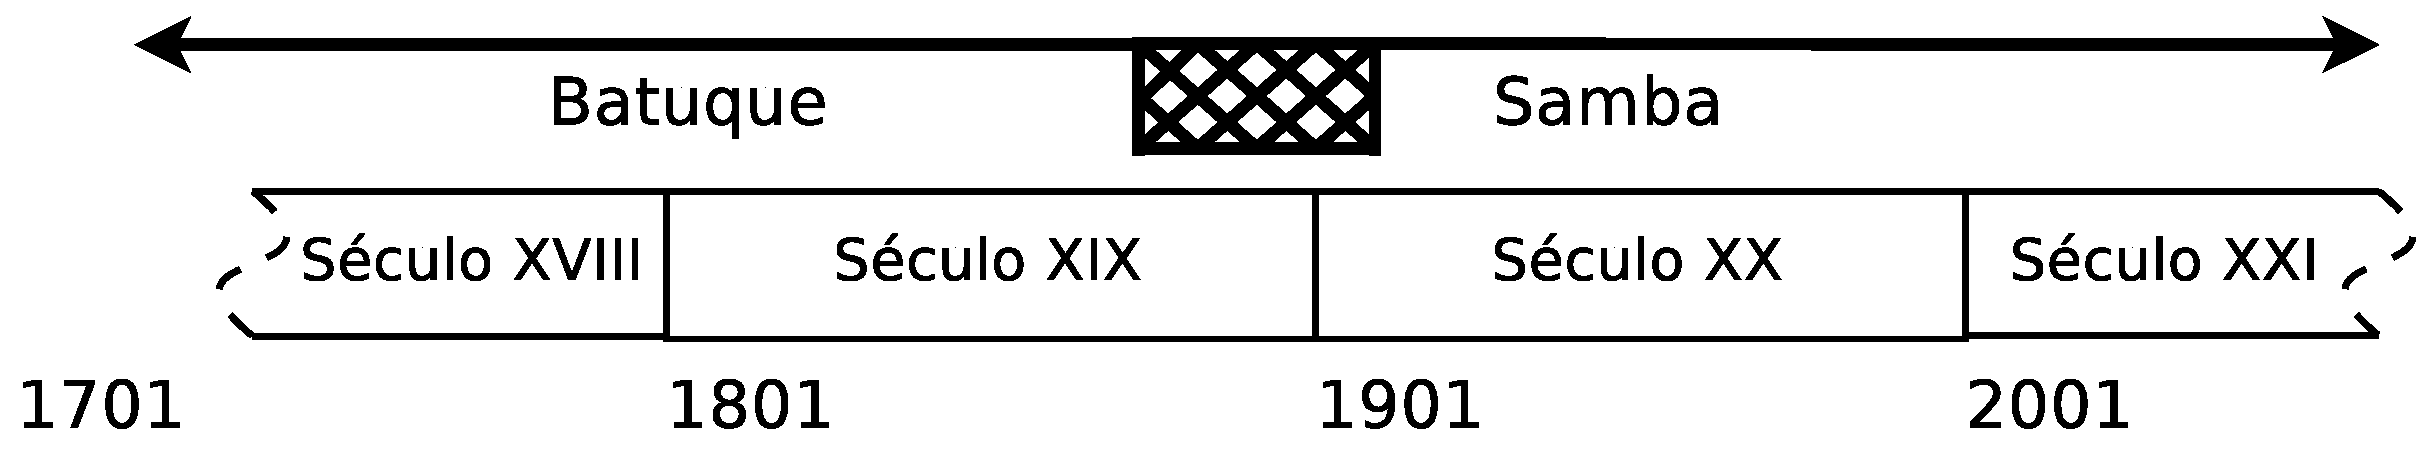
\includegraphics[width=0.85\textwidth]{chapters/cap-historia-samba/samba-crono.eps}
  \caption{Cronologia da designação geral dos festejos com danças, entendidas como com raiz africana.}
  \label{fig:sambacrono}
\end{figure}

\section{Expressões folclóricas relativas ao samba}

Para entender o folclore brasileiro, 
é importante ressaltar que o samba de roda, a batucada, 
o samba e o batuque são tipos gerais de dança afro-brasileira \cite[pp. 8]{reffolclorebatucadajornal} \cite[pp. 21]{jornalsambaderoda1}.
 
\begin{description}
\item [Samba de roda:]
\index{Samba de roda}
\index{Dança!Samba de roda}
\label{ref:Samba-de-roda-danca}
Também chamado, em 1936, \textbf{samba de morro} \cite[pp. 18]{jornalsambaderoda3}.
O samba de roda é uma manifestação cultural originaria da Baia que tem origem na dança dos negros do Brasil colonial \cite[pp. 21]{brasilpandeiro} \cite{silva2009capoeira},
esta se expandiu pelo Brasil todo e se popularizou nos estados de Rio de Janeiro e Pernambuco \cite{silva2009capoeira}.
No primeiro toque do tambor homens e mulheres se colocam a postos,
em circulo \cite[pp. 21]{brasilpandeiro} \cite{silva2009capoeira},
todo isto ao ritmo de orquestra de pandeiros, berimbaus, atabaque e agogô  \cite{silva2009capoeira}.
As personas passam ao centro e dançam individualmente ou em pares enquanto os demais batem palmas \cite[pp. 21]{brasilpandeiro}.
Um momento comum, em que a samba de roda e realizada é ao final das rodas da capoeira \cite{silva2009capoeira}.

Da união do \textbf{samba de roda} da Baia, com os ternos e ranchos de Reis, lusitano, 
e a música popular da época, 
nasceram as escolas de samba em Rio de Janeiro no segundo quartel no século XX \cite[pp. 8]{jornalsambaderoda4}

\item [Samba-de-umbigada:]
\index{Samba-de-umbigada}
\index{Dança!Samba-de-umbigada}
\label{ref:samba-de-umbigada}
Entre as danças ``profanas'' %\cite[pp. 85]{sandroni2001feitico} 
afro-brasileiras o gesto da umbigada é um elemento muito 
caraterístico \cite[pp. 32]{jornalsambaderoda2} \cite[pp. 85]{sandroni2001feitico},
de modo que em 1961 Edson Carneiro definiu e englobou as danças que realizam este 
gesto como ``samba-de-umbigada''; assim, tradições 
musicais como o samba de roda, o jongo, o lundu, o coco, o calango e o cateretê, 
seguindo Edson são englobadas com  ``samba-de-umbigada'' \cite[pp. 85]{sandroni2001feitico}.

\item [Batuque (1900s):]
\index{Batuque!1900s}
\index{Dança!Batuque (1900s)}
\label{ref:batuquedanca}
É uma dança catalogada como pertencente ao folclore brasileiro  \cite[pp. 96]{sandroni2001feitico} e
é realizada em roda, na qual participam dançarinos, músicos e espectadores \cite[pp. 89]{marcondes1977enciclopedia}.
Chama-se ``baixão'' à introdução ou preludio da dança  e é executada pelo violeiro  \cite[pp. 89]{marcondes1977enciclopedia}.
No centro da roda fica um dançarino solista ou um ou mais pares
que se incumbem na coreografia \cite[pp. 89]{marcondes1977enciclopedia},
onde todos dançam de forma separada \cite[pp. 65]{sandroni2001feitico}.
A dança consiste num forte marcado pelos quadris, sapateados, palmas e estalar de dedos  \cite[pp. 89]{marcondes1977enciclopedia}.
É uma dança de \textbf{umbigada} \cite[pp. 96]{sandroni2001feitico} \cite[pp. 89]{marcondes1977enciclopedia}, 
onde o dançarino ou dançarinos solistas
dão \textbf{umbigadas} nos figurantes da roda  escolhidos para substitui-los \cite[pp. 89]{marcondes1977enciclopedia}.



\item [Batucada (1900):]
\index{Batucada}
\index{Dança!Batucada}
\label{ref:batucadadanca}
No inícios do seculo XX,
a ``batucada'' se distingue de outros sambas-de-umbigada por seu componente violenta, 
sendo esta executada principalmente por homens \cite[pp. 8]{reffolclorebatucadajornal} \cite[pp. 103]{sandroni2001feitico};
este era um jogo de destreza corporal, variante da capoeira e da samba-de-umbigada,
onde existiam \textbf{pernadas} que tinham o objetivo de derrubar ao parceiro, o qual, ao se manter em pé apos a pernada,
ganhava o direito de escolher o próximo parceiro
 e consequentemente tinha o privilegio de dar a próxima pernada nele \cite[pp. 103]{sandroni2001feitico}.

Baile que usa instrumentos de percussão onde se cantam versos que são respondidos pelo coro;
seguindo os mestres do gênero, de Rio de Janeiro, 
não há batucada com instrumentos de corda e de sopro, 
e  todas são feitas em roda \cite[pp. 89]{marcondes1977enciclopedia}.
A origem do baile é provavelmente africana; porem, alguns autores acham que pode ter origem em  danças indígenas,
basando-se nos desenhos dos livros de Théodore de Bry (1528-1598) e
nas informações de cronistas coloniais como Jean de Léry (1534-1611) e
Hans Staden (fl.1547-1556) \cite[pp. 89]{marcondes1977enciclopedia}.


\item [Batucada (outras acepções a partir de 1930):]
\index{Batucada}
\index{Dança!Batucada}
\label{ref:batucadadanca1930}

A palavra batucada ganhou outra conotação a partir dos anos 1930 \cite[pp. 103]{sandroni2001feitico}.

Depois de 1930, se retiravam do carnaval baiano, três clubes de elite por motivos econômicos; 
nesse contexto emergiram as batucadas que ritualizavam a presença da cultura afro-mestiça no carnaval; 
nesse período, a nível social e politico, a batucada e o samba eram considerados centrais no carnaval; 
porem, apos a década 1950, com o ressurgimento dos clubes de elite foi fechada a ``Era das Batucadas'' \cite{ICKES2013}.\\



Por outro lado, uma descrição interessante é dada no coro da música ``É batucada'', 
de Caninha e Visconde de Bicoiba (Bicohyba), no dia 18 de dezembro de 1932 \cite[pp. 12]{refebatucadajornal}.
\begin{citando}
Samba do morro\\
Não é samba, é batucada.\\
É batucada!\\
É batucada! Oi ...\\
\end{citando}
Caninha e Bicoiba indicavam com esses versos que na cidade (Rio de Janeiro),
o samba era privilegio dos compositores de espírito comercial, 
como Donga quando registrou pelo telefone em 1916 \cite[Cad. B pp. 4]{jornalsambaderoda5},
e que o resto de compositores que saiam do morro o que faziam era batucada 
(entendida na época como mais primitiva).\\




Finalmente, no vocabulário informal falado no morro (RJ em 1959), 
chama-se  ``batucada''
quando se trata de fazer humor ou satirizar alguma coisa \cite[pp. 32]{jornalsambaderoda2}.
\end{description}

%%%%%%%%%%%%%%%%%%%%%%%%%%%%%%%%%%
%% MARACATÚ
%%%%%%%%%%%%%%%%%%%%%%%%%%%%%%%%%%


